\section{Liste des élements à installer}
\begin{itemize}
    \item Deux rails de leds IR.
    \item Un boitier étanche contenant: Le Rpi4, la caméra, le transformateur 12VDC-5VDC, le régulateur 1.5V, le jeu de relai et le fusible d'entrée.
    \item Tiroir pour la télécommande avec le jeu d'aimant de levage.
\end{itemize}
\section{Disposition prévue}
Comme indiqué dans le chapitre \ref{chap:exi}, nous avons possibilité d'utiliser le support perforé ainsi que la zone libre sur le timon.
Le principe est le suivant, fixer le boitier étanche à une plaque d'aluminium qui elle même sera fixer sur le support, ainsi, il sera plus simple
de placer le boitier selon les besoins.

La camera et son filtre seront placés dans le boitier et plaqués contre la facade transparente, de manière à observer la route entre le semoir
et le pick-up.

Les rails de leds IR seront placés de part et d'autre du timon à 80 \si{\centi\metre} du semoir en direction du pick-up pour "éclairer" le champ
de vue de la caméra. La fixation permettra aux deux rails de se replier sur le timon lorsque l'éclairage ne sera pas utilisé.

Le tiroir permettant de contrôler la télécommande sera placé sur le boitier étanche, celui-ci s'ouvrant de face, ça ne posera pas problème.

Les illustations suivantes permettent de se faire une idée plus précise de ce qui est prévu.

\begin{figure}[H]
    \centering
    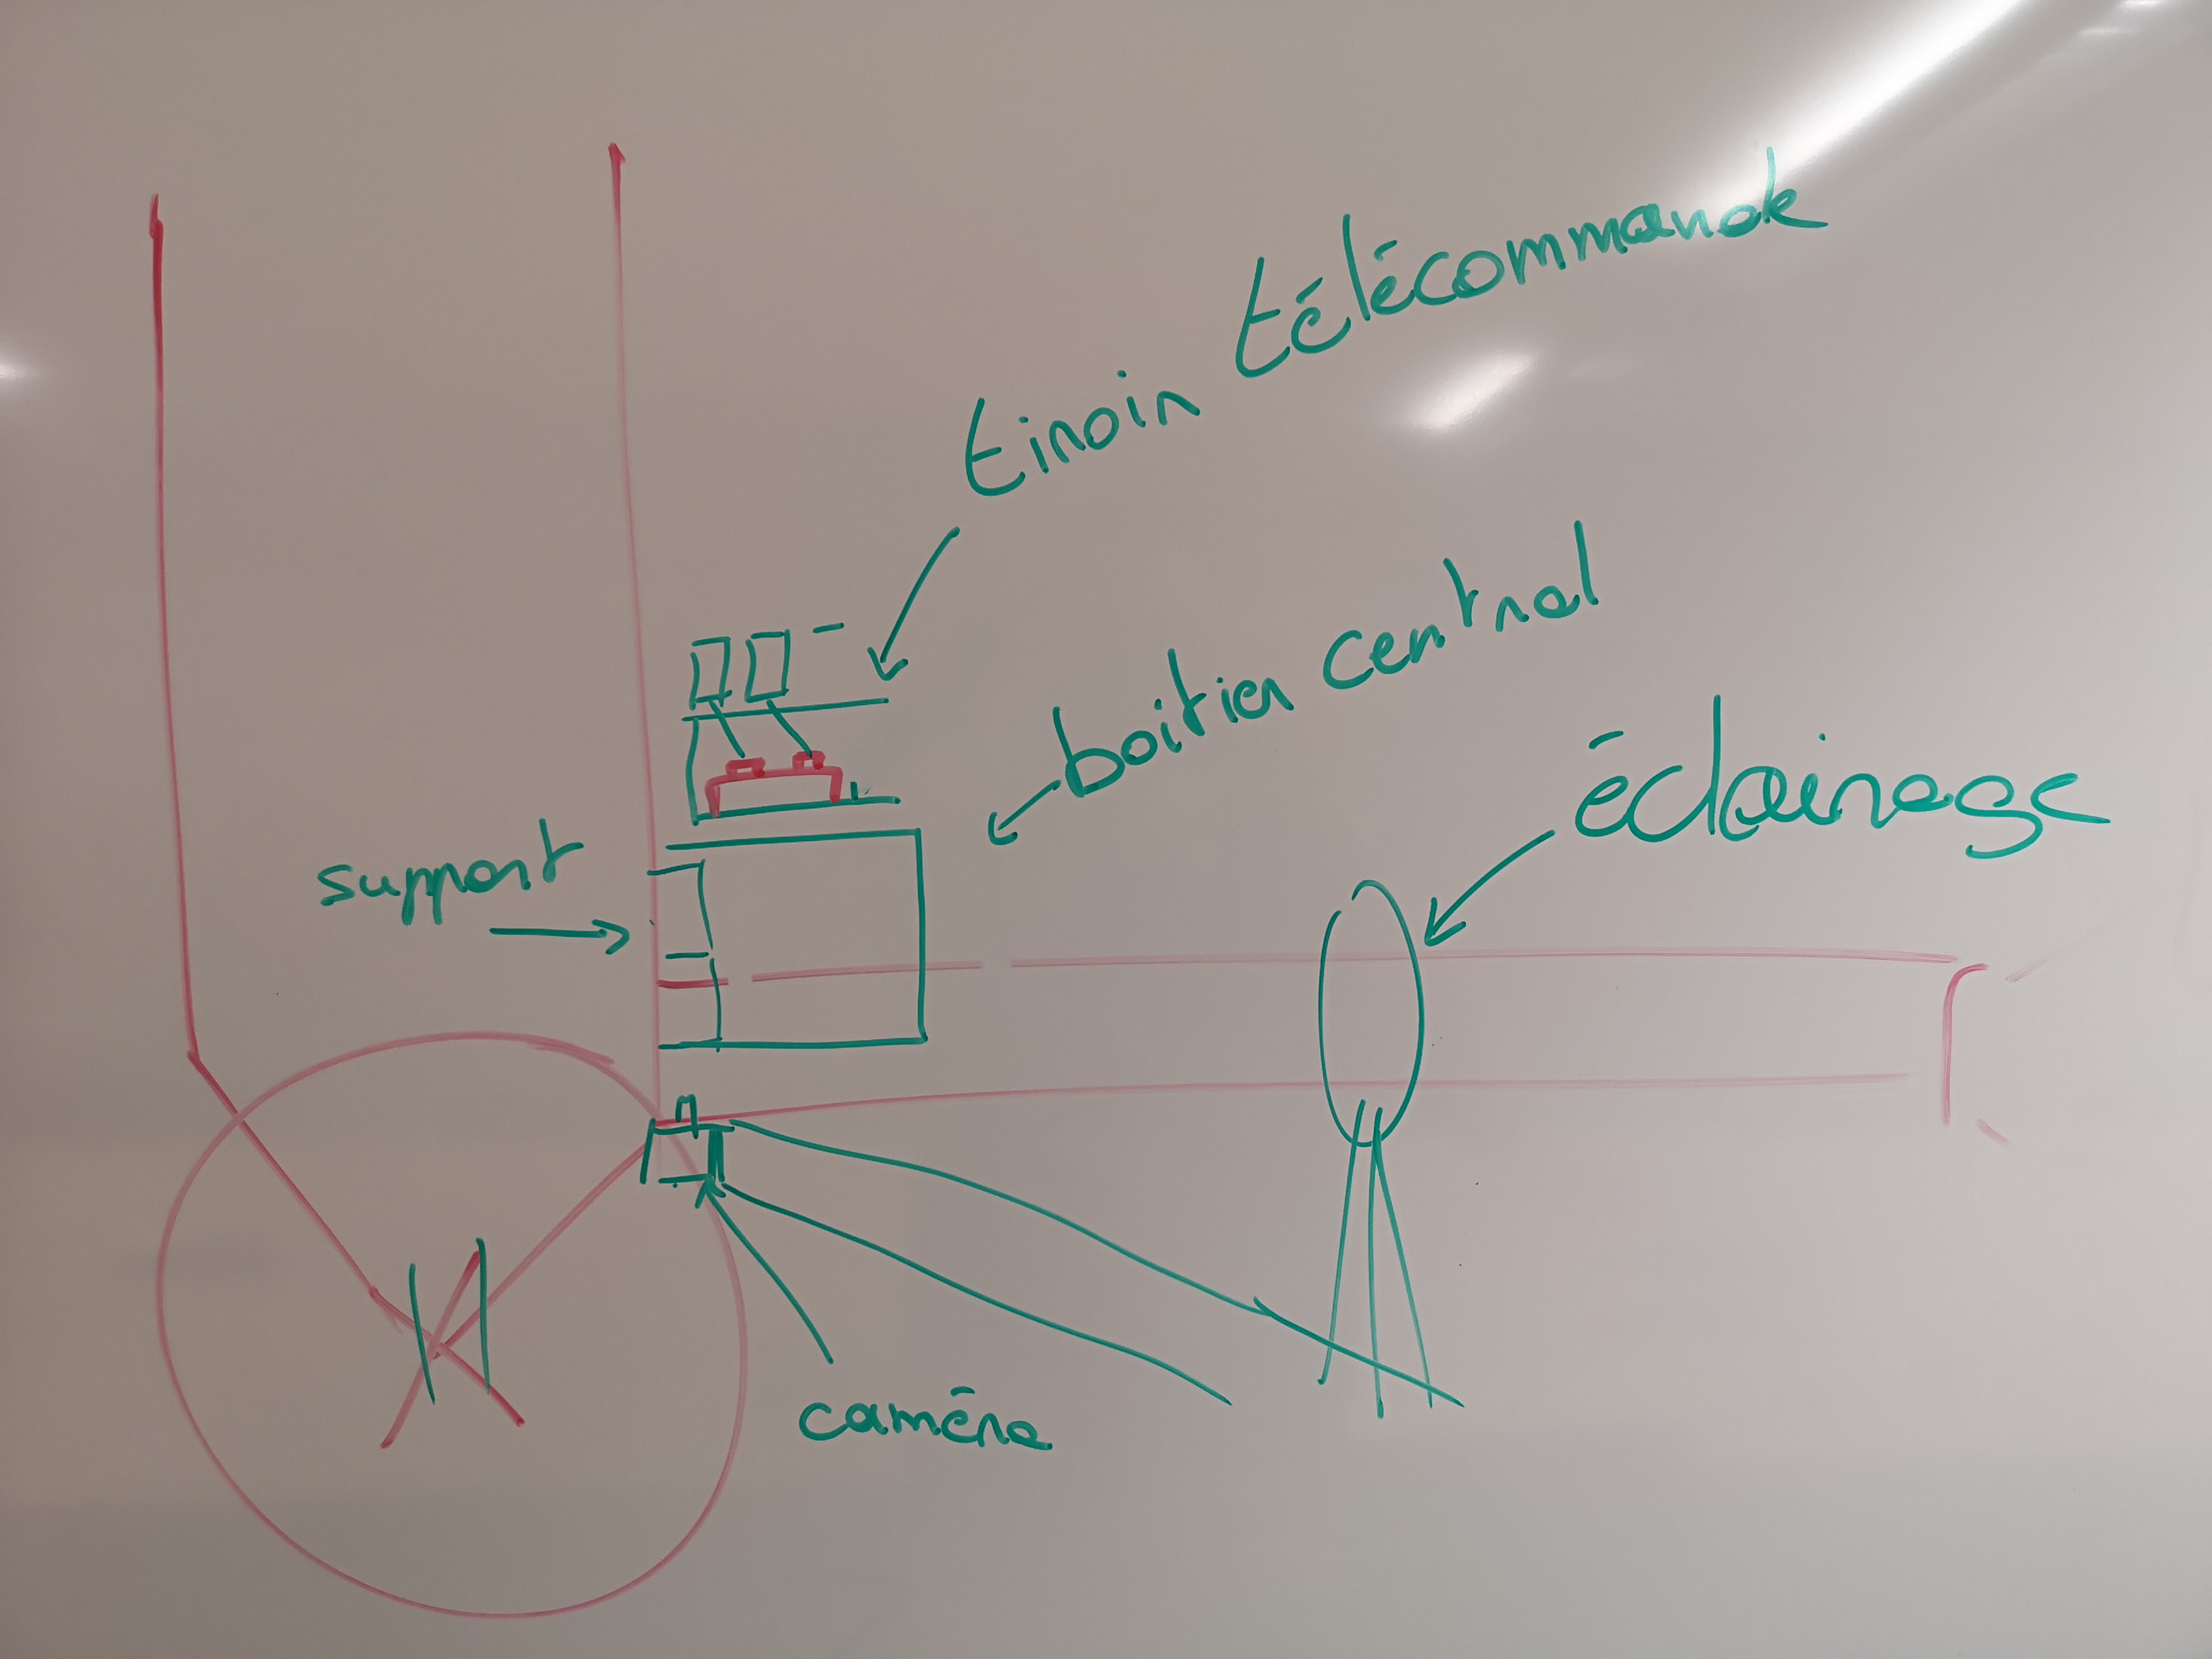
\includegraphics[height=7cm]{assets/figures/montage1.jpg}
    \caption{Montage prévu - Vue de côté}
\end{figure}

\begin{figure}[H]
    \centering
    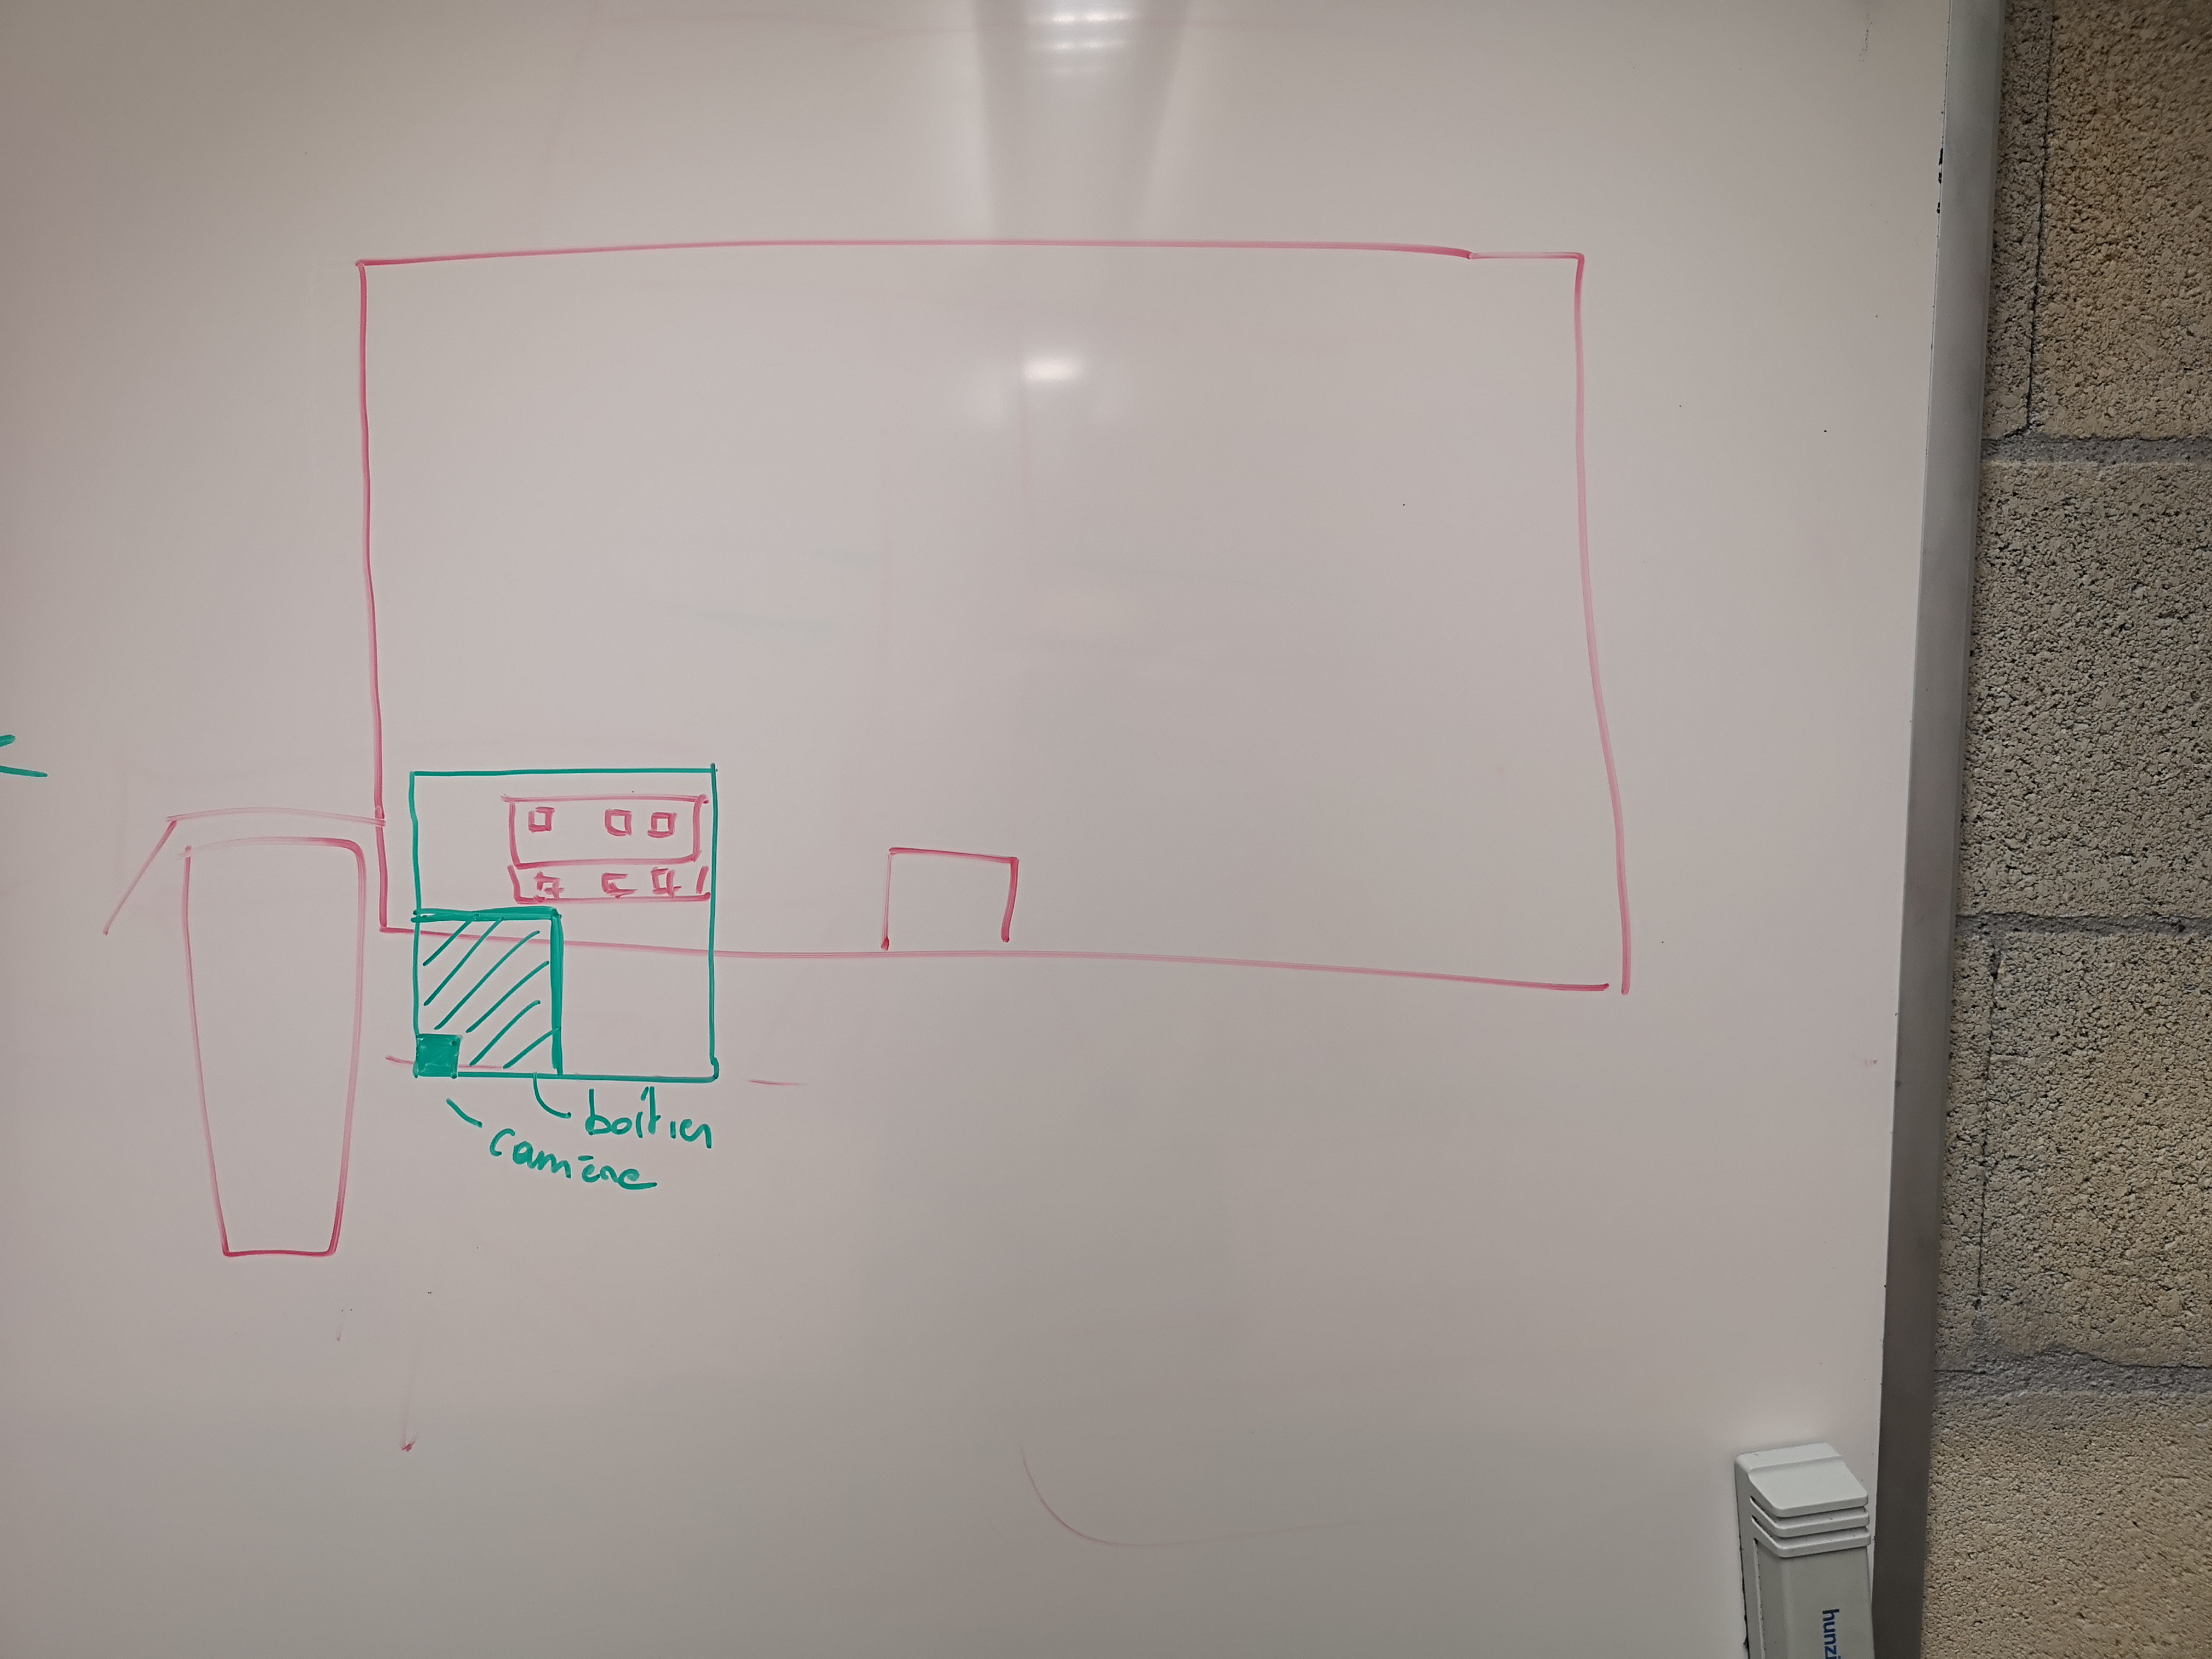
\includegraphics[height=7cm]{assets/figures/montage2.jpg}
    \caption{Montage prévu - Vue de face}
\end{figure}

\begin{figure}[H]
    \centering
    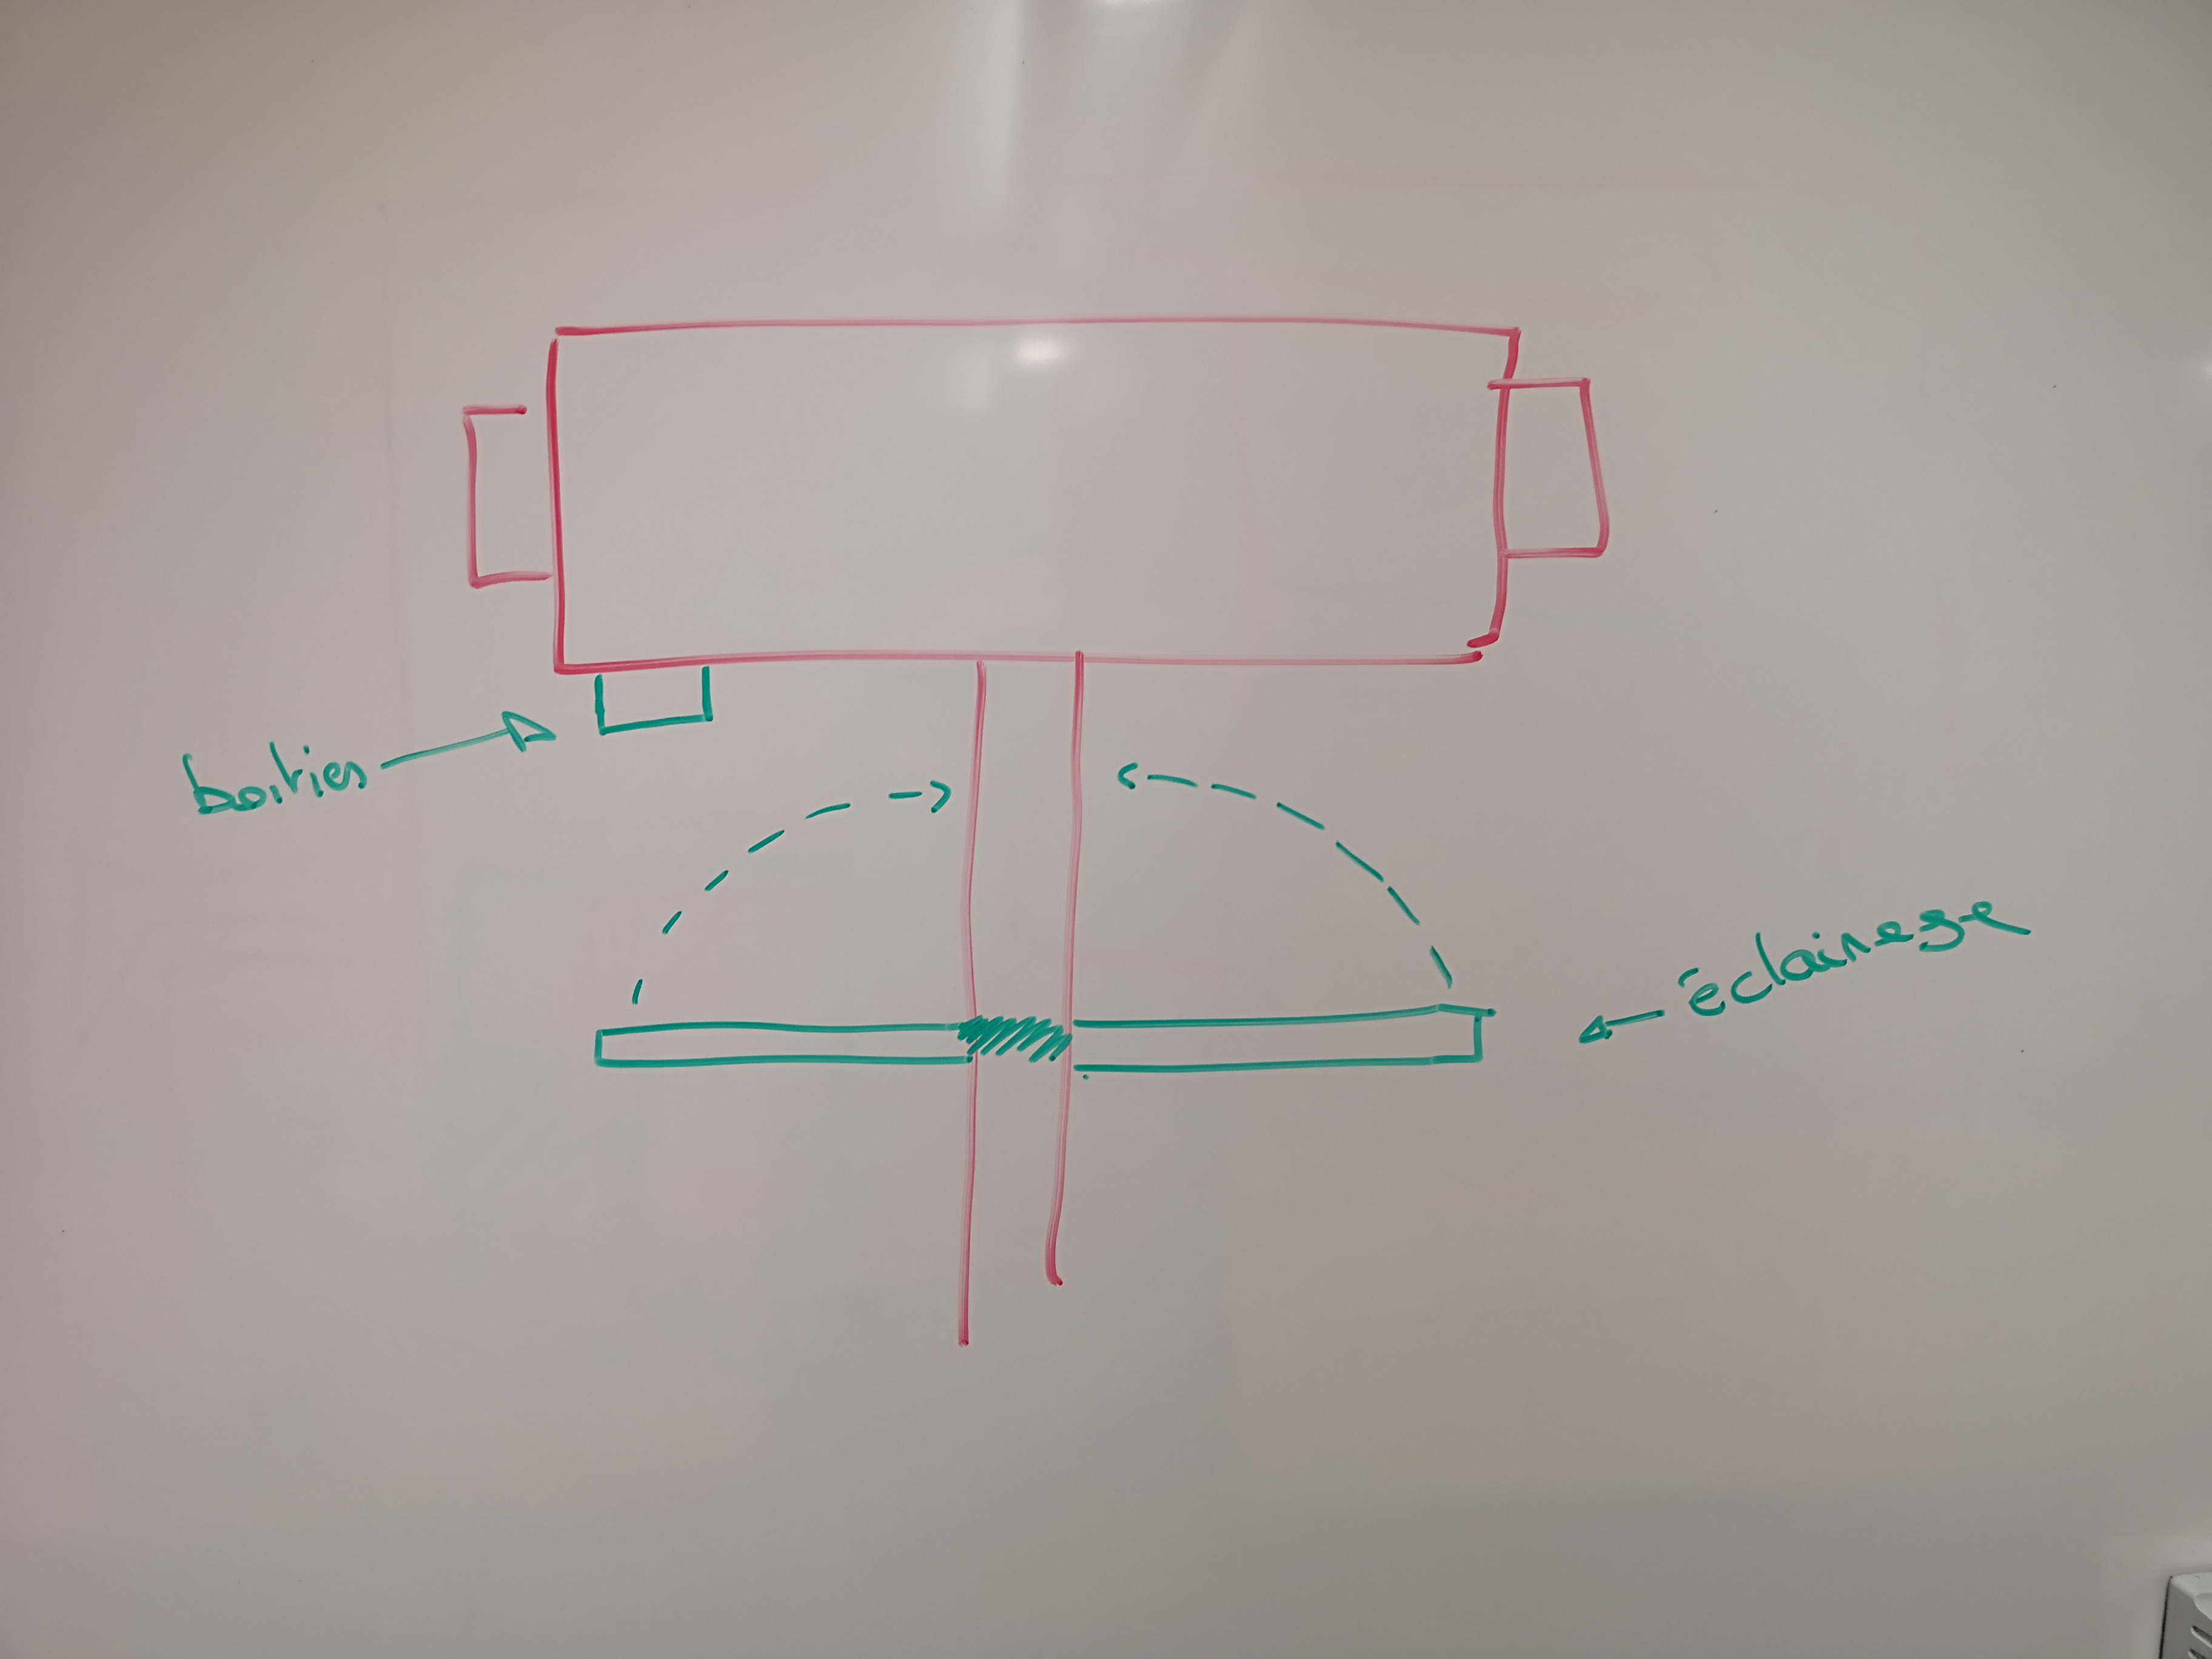
\includegraphics[height=7cm]{assets/figures/montage3.jpg}
    \caption{Montage prévu - Vue du dessus}
\end{figure}
\section{Installation finale}